% Preamble
\documentclass [11pt]{article}

\usepackage{setspace}
\usepackage{amssymb}
\usepackage{amsmath}
\usepackage{amsfonts}
\usepackage{amssymb}
\usepackage{setspace}
\usepackage{amsthm}
\usepackage{textcomp}
\usepackage{graphicx}
\usepackage{url}
\usepackage{color}
\usepackage[dvipsnames]{xcolor}
\definecolor{cuteBlue}{rgb}{0.258, 0.387, 0.574}
\definecolor{cuteGreen}{rgb}{0, 0.3, 0}
\usepackage{cancel}
\usepackage{comment}
\usepackage[framemethod=TikZ]{mdframed}
\usepackage{enumitem}
\usepackage{wasysym}
\usepackage{listings}
\usepackage{float}
\usepackage{booktabs}
\usepackage{fixltx2e}
\usepackage{threeparttable}
\usepackage{titling}
\usepackage{zref-base}
\usepackage{makecell}
\usepackage{array}
\usepackage{hhline}
\usepackage{titlesec}
\usepackage{gensymb}
\usepackage{caption}
\usepackage{subcaption}

% To make jumping between equation, figure, citation references easier
\usepackage[colorlinks=true, urlcolor=cuteBlue, citecolor=cuteGreen, linkcolor=black]{hyperref}

% To make caption labels (i.e. Figure 1, Figure 2...) bold and
% make all caption text small
\usepackage[labelfont=bf, font=small]{caption}

% For strike-out text during editing
\usepackage[normalem]{ulem}

%Latin accents
\usepackage[utf8]{inputenc}

%subfigures
\usepackage{caption}

% Add author affiliations
\usepackage{authblk}

% %%%%%%%%%%%%%%%%%%%%%%%%%%%%%%%%%%%%%%%%%%%%%%%%%%%%%%%%%%%%%%%%%%%%%%%%%%%%%%
% %%%%%%%%%%%%%%%%%%%%%%%%%%%%%%%%%%%%%%%%%%%%%%%%%%%%%%%%%%%%%%%%%%%%%%%%%%%%%%

% Margins and spacings
\setlength{\evensidemargin}{0.0cm}
\setlength{\oddsidemargin}{0.0cm}
\setlength{\topmargin}{-2.0cm}
\setlength{\textwidth}{17cm}
\setlength{\textheight}{22cm}
\setlength{\parskip}{2.5mm}
\reversemarginpar
\marginparsep  0.1in
\marginparwidth 0.7in

% Give more spacing in equation arrays
\setlength{\jot}{10pt}

% Allow page breaks in multiline equations
\allowdisplaybreaks

% Set up title spacing so we don't waste so much space
\setlength{\droptitle}{-8em}
\date{\vspace{-5em}}  % No date will appear in title.

% Spacing between section headings and text
\titlespacing\section{0pt}{12pt plus 4pt minus 2pt}{-2pt plus 2pt minus 2pt}
\titlespacing\subsection{0pt}{12pt plus 4pt minus 2pt}{-2pt plus 2pt minus 2pt}
\titlespacing\subsubsection{0pt}{12pt plus 4pt minus 2pt}{-2pt plus 2pt minus 2pt}

% Convenient micron symbol
\newcommand{\micron}{{\textmu}m}

% No excess spacing for lists
\setlist{itemsep=0pt, topsep=0pt}

% Allow paragraph indentations in lists
\setitemize{listparindent=\parindent}
\setenumerate{listparindent=\parindent}

% Column type for tables with nice spacing
\newcolumntype{M}[1]{>{\centering\arraybackslash}m{#1}}
\newcolumntype{N}{@{}m{0pt}@{}}

% Easier equation writing
\newcommand{\RM}[1]{\mathrm{#1}}
\newcommand{\purple}[1]{\textcolor{purple}{#1}}


% %%%%%%%%%%%%%%%%%%%%%%%%%%%%%%%%%%%%%%%%%%%%%%%%%%
% Document settings
% %%%%%%%%%%%%%%%%%%%%%%%%%%%%%%%%%%%%%%%%%%%%%%%%%%

% References
\usepackage[
	backend=bibtex,
	style=phys, 
	sorting=none,				% Do not sort bibliography
	url=false, 					% Do not show url in reference
	doi=false, 					% Do not show doi in reference
	isbn=false, 				% Do not show isbn link in reference
	eprint=false, 			% Do not show eprint link in reference
	maxbibnames=9, 			% Include up to 9 names in citation
	firstinits=true,
]{biblatex}
% Add library
\addbibresource{./regseq_refs}

% Bold the 'Figure #' in the caption and separate it from the title/caption
% with a period
% Captions will be left justified
\usepackage[
	aboveskip=30pt,
	belowskip=10pt,
	labelfont=bf,
	labelsep=period,
	justification=raggedright,
	singlelinecheck=off
]{caption}

% Add numbered lines
\usepackage{lineno}
\linenumbers

\usepackage{textgreek}

% Package to include multiple title pages
% This will allow me to add a tile to the main text and to the SI
\usepackage{titling}

% This package will allow me to define booleans to compile main text or SI
\usepackage{ifthen}
\newboolean{maintext}
\newboolean{sitext}

%%%%%%%%%%%%%%%%%%%%%%%%%%%%%%%%%%%%%%%%%%%%%%%%%%%%
% Personalized functions
%%%%%%%%%%%%%%%%%%%%%%%%%%%%%%%%%%%%%%%%%%%%%%%%%%%%
% Commenting
\newcommand{\rp}[1]{\textcolor{red}{(RP:~#1)}} % Commenting
\newcommand{\tr}[1]{\textcolor{purple}{(TR:~#1)}} % Commenting

% To define more useful LaTeX commands
\usepackage{xparse}

% Define command to begin the supplementary section
\newcommand{\beginsupplement}{
				\setcounter{section}{0} % Restart section counter
        \renewcommand{\thesection}{S\arabic{section}}%
        \setcounter{table}{0} % Restart table counter
        \renewcommand{\thetable}{S\arabic{table}}%
        \setcounter{figure}{0} % Restart figure counter
        \renewcommand{\thefigure}{S\arabic{figure}}%
        \setcounter{equation}{0} % Restart equation counter
        \renewcommand{\theequation}{S\arabic{equation}}%
     }

%%%%%%%%%%%%%%%%%%%%%%%%%%%%%%%%%%%%%%%%%%%%%%%%%%%%
%% Begin document
%%%%%%%%%%%%%%%%%%%%%%%%%%%%%%%%%%%%%%%%%%%%%%%%%%%%

\title{\textbf{Another 100 genes}}
% Authors
\author[1]{Tom R\"oschinger}
\author[1]{Grace Solini}
\author[2]{Anika Nawar Choudhury}
\author[2, 3, 4]{Stephen Quake}
\author[1, 5, +]{Rob Phillips}

% Affiliations
%\affil[*]{Equal Contribution}
\affil[1]{Division of Biology and Biological Engineering, California Institute
of Technology, Pasadena, CA 91125, USA}
\affil[2]{Chan Zuckerberg Biohub, San Francisco, CA 94158, USA}
\affil[3]{Department of Bioengineering, Stanford University, Stanford, CA 94305, USA}
\affil[4]{Department of Applied Physics, Stanford University, Stanford, CA 94305, USA}
\affil[5]{Department of Physics, California Institute of Technology, Pasadena,
CA 91125, USA}
\affil[+]{Correspondence: phillips@pboc.caltech.edu}

% date
% \date{\today}

\setcounter{Maxaffil}{0}
% Set affiliations in small font
\renewcommand\Affilfont{\itshape\small}

\begin{document}
%% MAIN TEXT

% Remove main text from the table of contents by specifying not to include
% any section or subsection
\addtocontents{toc}{\protect\setcounter{tocdepth}{-1}}


	% Define reference segment for main text
	\begin{refsegment}
	% Generate filter to not include references from main text in the
	% supplemental references

		\defbibfilter{notother}{not segment=\therefsegment}
		% Set boolean to ether compile or not the main text
		\setboolean{maintext}{true}
		\ifthenelse{\boolean{maintext}}{
		\maketitle % Set title for paper


		%% !TEX root = ./main.tex
\section{Abstract}


		% !TEX root = ./main.tex
\section{Introduction}
It has been more than sixty years since Jacob and Monod \cite{jacob1961genetic} shaped the way we think about transcriptional regulation in prokaryotes, yet, although more than one trillion bases have been stored in the NIH database \tr{find right citation format}, we have yet to obtain a full understanding of how all the genes of a single organism are regulated. Even in the case of one of biology's best studied model organism, \textit{Escherichia coli}, about two thirds of the genes lack any regulatory annotation \tr{add section to supp with details}. For other prokaryotic model organisms the numbers are similar, while higher order model organisms such as \textit{Saccharomyces cerevisiae} and \textit{C. elegans} have close to no regulatory annotations, given the arguably more complex nature of gene regulation in eukaryotes \tr{also add section to supp for these organisms}. Understanding how genes are regulated is required to understand how an organism adapts its physiology on short time scales to environmental stresses, as well as evolutionary adaption on long time scales. In addition, gene regulation networks and their building blocks, such as transcription factor binding sites and RNA polymerase (RNAP) promoters, are key elements in the design of synthetic gene circuits \tr{cite something here too, guess there is a ton. Repressilator?}.

With its ever increasing availability, Next Gen Sequencing (NGS) is primed to be the method of choice to discover transcription factor and RNAP binding sites. A vast array of methods exists that make it possible to identify binding sites of either specific proteins \tr{cite} or for a broad spectrum of DNA binding factors \tr{cite}. In methods like ChIP-Seq \cite{rhee2012chip}, proteins have to be cross linked to DNA, which does not work for all transcription factors, such as LacI in \textit{E. coli} \tr{cite}. While the resolution of these methods is ever improving, it does not allow for a nucleotide resolution yet \tr{cite}, making it difficult to identify changes in binding affinity caused by single mutations. Other methods such as ATAC-seq \cite{buenrostro2015atac, li2019identification} and DNase-Seq \cite{boyle2008high} rely on open chromatin for binding site identification, and are therefore limited to mostly eukaryotic organisms \tr{look deeper for possible applications in bacteria, haven't found them yet}. Another approach is to use RNA-seq as readout for mutagenised promoter regions, where binding sites are identified as regions that, when mutated, lead to significant increase or decrease in expression of a repressor gene \cite{urtecho2018systematic, urtecho2020genome, ireland2020deciphering}. 

Here we present the regulatory architecture of x \tr{depends on how many we end up showing} genes, including energy matrices with nucleotide resolution that make it possible to build thermodynamic models to predict gene expression \cite{kinney2010using,belliveau2018systematic,barnes2019mapping,ireland2020deciphering}. Additionally, we present major improvements to the method called Reg-Seq \cite{ireland2020deciphering}, making further steps towards obtaining a method allowing to discover regulatory architectures genome wide. Reporter genes are chromosomally integrated into the \textit{E. coli} genome, and reduced diversity in mRNA stability lead to more precise identification of binding sites. A vast array of growth conditions is used to show how certain binding sites can only be identified in a certain growth condition, such as \tr{name example}. The identification of transcription factors was moved away from laborious mass spectrometry experiments, using \textit{in vitro} binding assays as well as a library of transcription factor knockout strains. Finally, improved computational analysis increases the speed of data analysis and the accuracy of parameters that are used for thermodynamic models \tr{here I am thinking Rosalinds stuff}.

\tr{paragraph about scaling to 1000}



		%% !TEX root = ./main.tex
\section{Methods}
\subsection{Promoter sequence import}
\subsection{Reporter construct design}
\subsection{Barcode Mapping}

\subsection{Genome Integration}
		%% !TEX root = ./main.tex
\section{Results}
\subsection{Genes studied}
\tr{Does this belong into results or introduction?}
In total we present the regulatory architecture of x promoters, which tells us how a total of y genes are regulated. 18 promoters were chosen as so called "gold standards". These genes have well annotated promoters and have been studied in detail in previous experiments \cite{belliveau2018systematic,ireland2020deciphering}. Including this set of genes allows us to compare the method presented in this work to previous iterations and verify the results, as well as find possible derivations or improvements. x promoters were chosen for genes that have been identified to have a high variation in protein copy number \tr{Probably should show that in the SI} across a set of 22 growth conditions by Schmidt et al., 2016 \cite{schmidt2016quantitative}. These genes were chosen since a high variation in copy number suggests that there are regulatory proteins controlling the expression of the gene. From the same dataset, a set of x promoters was chosen for genes with unidentified function, as annotated by the Schmidt et al., 2016 \cite{schmidt2016quantitative}. None of these promoters had any regulatory annotation prior to the experiments. Another set of x promoters were chosen for genes that were identified in EcoCyc as not having any functional annotation. Two groups of genes, so called iModulons \cite{lamoureux2021precise} were chosen from the work of Lamoureux et al. 2021, where ca. 800 RNA-Seq datasets were evaluated to find genes that were regulated in a distinct network. \tr{Give details for iModulons and their function in their respective paragraphs?} The \tr{Give summary of all genes at the end of this paragragh.}
\tr{Continue with genes of defined circuits and toxin/antitoxin genes}

\subsection{Barcode Mapping}
For each gene studied here, we designed a library of 1500 mutated promoter variants with an average mutation rate of 0.1 for each promoter that was identified with the gene in EcoCyc. If a gene did not have a promoter identified, we first looked for a possible TSS identified by Urtecho et al., 2018 \cite{urtecho2018systematic}, which then was taken as initial sequence for generating mutated variants. In some cases, no TSS could be identified and we used the model of LaFleur et al., 2022 \cite{lafleur2022automated}, which predicts trancsription start site given a genomic sequence of \textit{E. coli}, to find the site in the intergenic region leading up to the first coding region in the operon the gene was part of that had the highes predicit affinity for $\sigma70$-factors. A total of 178619 sequences were ordered from Twist Biosciences. We added random barcodes to the sequences and cloned them into a plasmid vector for amplification and subsequent cloning steps. Details can be found in Supplementary information sections \ref{sec:ident_tss}, \ref{sec:comp_prom_muta}, \ref{sec:library_cloning} and  \ref{sec:barcode_mapping}. 170192 (>95\%) of sequences were identified in the plasmid library (Figure \ref{fig:num_uniq_prom_var}), and an addional 17114 sequences were found, likely due to errors in the synthesis process of the oligonucleotide library. 


\subsection{Genome Integration of Reporters}




\subsection{Transcription Factor identification}
\subsection{Growth Conditions}
\begin{figure}
    \centering
    \includegraphics{../figures/FIG2.pdf}
    \caption{Method summary}
    \label{fig:method_sum}
\end{figure}
\subsection{Gold Standard genes}
\subsection{Ethanol iModulon}
YgeV has been predicted to be a regulator involved in purine catabolism, leading to the production of allantoin, which can be used as a sole nitrogen source \cite{iwadate2019identification}. There are 16 putative regulatory targets \cite{lamoureux2021precise} for YgeV, including the \textit{xdhABC} operon, which degrades xanthine to uric acid \cite{iwadate2019identification} in the purine catabolism pathway. \textit{E. coli} can survive exposure to low ethanol concentrations up to 5\%, which can even lead to increased DNA synthesis \cite{basu1994effect}, but mostly leads to varies stress responses such as an increased production of ROS. Growth in media supplemented with ethanol induced a change in gene expression for genes regulated by YgeV in a \textDelta\textit{baeR} or \textDelta\textit{cpxR} mutant strain. \tr{Is there a correlation between ethanol response and higher need for nitrogen?}
\subsection{Oxidative stress response iModulon}
The putative transcription factor YmfT regulates 14 out of 23 genes in the e14 prophage and is predicted to respond to oxidative stress \cite{lamoureux2021precise}. Oxidative stress is caused by reactive oxygen species (ROS) such as $\text{H}_2\text{O}_2$, which are highly reactive and damage DNA, the cell wall, proteins \cite{ezraty2017oxidative} etc., however, oxidized amino acids can also lead to confirmational changes in transcription factors, such as OxyR and HypT, which induce DNA binding and subsequent regulation of genes involved in response to oxidative stress  \cite{ezraty2017oxidative}. Hydrogen peroxide is produced endogenously in various pathways in \textit{E. coli} and especially in high amounts when phenylethylamine is used as either carbon or nitrogen source \cite{ravindra2013escherichia}, hence we used used minimal media supplemented with 10 mM 2-phenylethylamine hydrochloride (PEA) as sole carbon source to induce stress responses to $\text{H}_2\text{O}_2$ and therefore oxidative stress. \tr{discuss findings of ymfT modulon and how it relates to oxyR, look at oxyR iModulons and possibly do another run including this gene.}
\subsection{Antitoxin/Antibiotic genes}
\subsection{other y-ome genes}

		%% !TEX root = ./main.tex
\section{Discussion}
\begin{itemize}
    \item discuss how to scale to 1000 genes
\end{itemize}

		%% !TEX root = ./main.tex
\section{To do list}
\begin{itemize}
    \item Write Introduction
    \item Collect references from reg-seq paper and new references
    \item write paragraphs about genes chosen
    \item 
\end{itemize}

		}{}% Close boolean to compile main text
		% Print main text references
		\printbibliography[segment=\therefsegment]
		% Close reference segment
	\end{refsegment}

\clearpage

% Set title for supplemental information
\title{\textbf{Supplemental Information for: Whatever the title will be}}
% \date{}


\setboolean{sitext}{true}
\ifthenelse{\boolean{sitext}}{
\maketitle

% SUPPLEMENTAL MATERIAL

% Indicate that now all sections and subsections should be included in the
% table of contents so that only the SI is included.
\addtocontents{toc}{\protect\setcounter{tocdepth}{2}}

	% Define reference section for the supplemental material
	\begin{refsegment}
		% Set equation, table and figure counters to begin with "S"
		\beginsupplement
		% \tableofcontents
		%% !TEX root = ./main.tex
\section{Finding number of genes without regulatory annotation} \label{sec:reg_ignorance}
\subsection{\textit{E. coli} K12 MG1655}
\subsection{\textit{Bacillus Subtilis}}
\subsection{\textit{Pseudomonas Aeruginosa}}
\subsection{\textit{Saccharomyces cerevisiae}}
\subsection{\textit{Drosophila Melanogaster}}
\subsection{\textit{C. elegans}}

		%% !TEX root = ./main.tex
\section{Reporter Sequence design}

		%% !TEX root = ./main.tex
\section{Oligo Pool Design} \label{sec:oligo_pool}
\subsection{Identification of Transcription Start Sites}
All oligo pools used in this work were manually designed. For each gene in our list we looked for promoters in Ecocyc \cite{keseler2010ecocyc} (accessed 12/08/2021) using the transcription start site if the promoter was found. If multiple promoters were identified, each promoter was included in the experiment. If no promoter was found, we looked for transcriptionally active sites in the data set from Urtecho et al, 2020\cite{urtecho2020genome}. In their work, every part of the genome was tested for transcription initiation in LB. If we could find a site that was identified as active close to the gene of interest, we chose this site as origin for computational promoter mutagenisis. If no transcription start site could be identified for a gene, the model from \cite{la2021automated} was used to computationally predict a transcription start site in the intergenic region. The site predicted to be the most active within 500 bp upstream of the coding region was chosen as transcription start site since more than 99\% of transcription start sites are within that region in \textit{E. coli} K12 MG1655, see Fig.~\ref{fig:tss_distance}. Restriction enzymes leaving compatible sticky ends to the digested plasmid were used to cut the RiboJ::sfYFP element.  

\begin{figure}
    \centering
    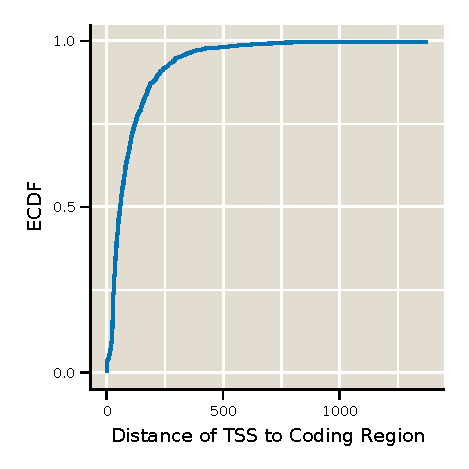
\includegraphics{../figures/tss_CR_distance.pdf}
    \caption{ECDF of distances of transcription start sites to the coding region for every operon in \textit{E. coli} that has a transcription start site annotated in EcoCyc. }
    \label{fig:tss_distance}
\end{figure}


\begin{figure}
    \centering
    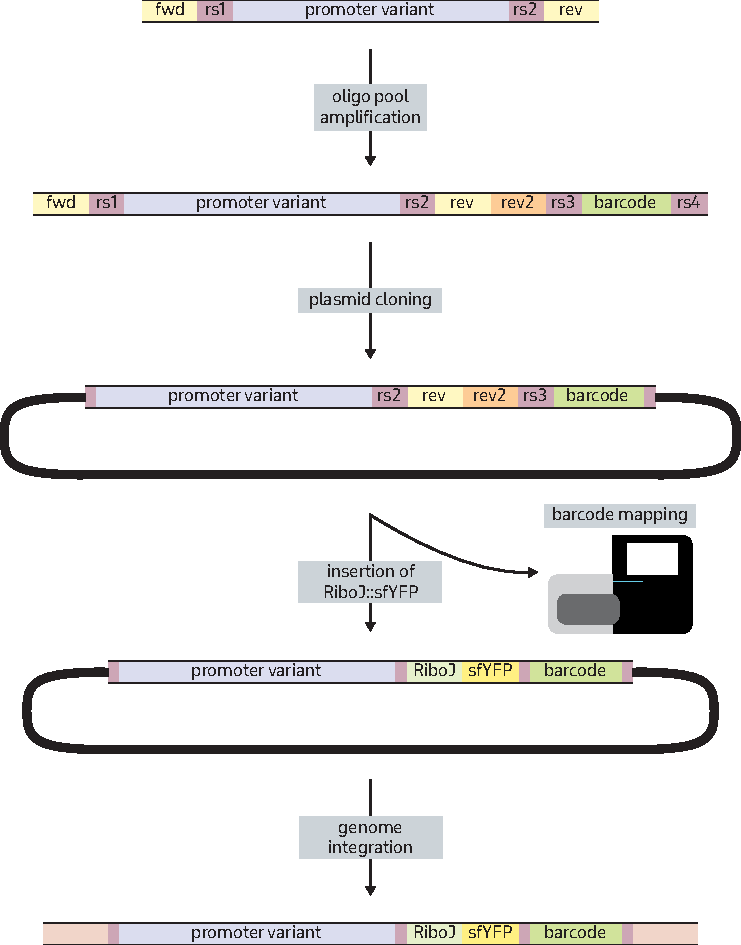
\includegraphics{../figures/cloning_scheme.pdf}
    \caption{Placeholder figure for cloning scheme.}
    \label{fig:cloning}
\end{figure}

\subsection{Computational Promoter Mutagenesis}
Once a TSS is identified, the 160 bp region from 115 bp upstream of the TSS to 45 bp downstream is taken from the genome. It has been shown that most cis-regulation is happening within this window \cite{rydenfelt2014statistical}. Based on the approach by \cite{kinney2010using}, each promoter sequence is mutated randomly at a rate of 0.1 per position. 1500 mutated sequences are created per promoter, following the approach from \cite{ireland2020deciphering}, which creates sufficient mutational coverage across the window. The promoter oligonucleotides are flanked by restriction enzyme sites (\textit{rs1} and \textit{rs2} in Fig.~\ref{fig:cloning}) that are used in downstream cloning steps. The restriction sites are flanked by primer sites used to amplify the oligo pool. Primer sequences were chosen from a list of orthogonal primer pairs, designed to be optimal for cloning procedures \cite{subramanian2018set}. oligo pools were synthesized (TwistBioscience, San Francisco, CA, USA) and used for subsequent cloning steps.


\section{Library Cloning}
\subsection{Cloning oligo pool into plasmid vector}
\label{sec:library_cloning}
The oligo pool was amplified using a 20bp forward primer (SC142) and a 40 bp reverse primer (SC143), which consists of 20bp primer binding site and 20bp overhang. PCR amplifications were run to minimal amplification to minimize amplification bias. PCR products were cleaned and concentrated (DNA Clean \& Concentrator-5, ZymoResearch) and used for a second amplification step. The 20 bp overhang from the first amplification was used as primer site for a reverse primer (SC172), which contains randomized 20 bp barcode, flanked by two restriction enzyme sites (\textit{rs3} and \textit{rs4} in Fig.~\ref{fig:cloning}). The forward primer is the same as in the first amplification step. PCR amplification is run again to minimal amplification to minimize amplification bias. PCR products are run on a 2\% agarose TAE gel and subsequently extracted and purified (Zymoclean Gel DNA Recovery Kit, ZymoResearch). In the next step, restriction digest is performed on the outer restriction enzyme sites (\textit{rs1} and \textit{rs4} in Fig.~\ref{fig:cloning}). Unless noted otherwise, all restriction digests were run for 15 minutes at 37C. The plasmid vector was digested with different restriction enzymes which create compatible sticky ends. Most restriction enzyme sites are palindromes, so by choosing different enzymes with compatible ends, we avoid having palindromes flanking the plasmid inserts. This is important, since these sites are used for amplifications in the library preparation steps later in the protocol. (\purple{Maybe not needed to say}). The oligo pool is combined with the plasmid vector using T7 DNA ligase (New England Biolabs, Ipswich, MA, USA) following the suppliers protocol. Ligation products were cleaned and concentrated (DNA Clean \& Concentrator-5, ZymoResearch) and drop dialysis (MF-Millipore VSWP02500, MilliporeSigma, Burlington, MA, USA)  was performed for 1h to improve sample purity. Electroporation using \textit{E. coli} pir116 electrocompetent cells (Lucigen, Middleton, WI) was performed at 1.8kV in 1mm electroporation cuvettes, followed by 1h recovery at 37C and 250rpm in 1 ml LB-media (\purple{details here}, the same for all following mentionings of LB). The entire cultures were plated on 150mm kanamycin (50$\mu$g/ml) + LB petri dishes and grown overnight. The following day, plates were scraped and the colonies resuspended. Freezer stocks were prepared using a 1:1 dilution of resuspended colonies and 50\% glycerol. Cultures were inoculated with $5\times 10^8$ cells in 200ml of LB + kanamycin (50$\mu$g/ml) and grown at 37C until saturation. Plasmid was extracted (ZymoPURE II Plasmid Maxiprep Kit, ZymoResearch) and used subsequent sequencing (see \ref{sec:barcode_mapping}). The plasmid library is then used as template in a restriction digest using restriction enzymes $rs2$ and $rs3$. The resulting product was cleaned and concentrated (NEB Monarch) and concentration measured on a Nanodrop. Similarly, the riboJ::YFP element was PCR amplified (primers SC191 and SC192), adding restriction sites as overhangs (see table \ref{tab:re_sites}). The PCR product was cleaned and concentrated (NEB Monarch) and digested with the respective restriction enzymes. The plasmid library is combined with the RiboJ::sfYFP element using 7 DNA ligase (New England Biolabs, Ipswich, MA, USA) following the suppliers protocol. Ligation products were cleaned and concentrated (NEB Monarch) and drop dialysis (MF-Millipore VSWP02500, MilliporeSigma, Burlington, MA, USA)  was performed for 1h to improve sample purity. Electroporation using \textit{E. coli} pir116 electrocompetent cells (Lucigen, Middleton, WI) was performed at 1.8kV in 1mm electroporation cuvettes, followed by 1h recovery at 37C and 250rpm in 1 ml LB-media. The entire cultures were plated on 150mm kanamycin (50$\mu$g/ml) + LB petri dishes and grown overnight. The following day, plates were scraped and the colonies resuspended. Freezer stocks were prepared using a 1:1 dilution of resuspended colonies and 50\% glycerol. Cultures were inoculated with $5\times 10^8$ cells in 200ml of LB + kanamycin (50$\mu$g/ml) and grown at 37C until saturation. Plasmid was extracted (ZymoPURE II Plasmid Maxiprep Kit, ZymoResearch) and used for subsequent genome integration. 


\section{Barcode Mapping}
\label{sec:barcode_mapping}
The plasmid library is used for barcode mapping. Purified plasmid is PCR amplified using forward primer (SC185) outside the promoter region and a reverse primer outside the 20bp barcode (SC184). The PCR is run to minimal amplification (until a band is visible on an ararose gel), and the product is gel purified (NEB Monarch). The purified DNA was used as template for a second PCR using a primer (SC196) adding an Illumina P5 adapter to the promoter side, and a primer (SC199) adding an Illumina P7 adapter. The PCR is again run to minimal amplification and gel purified (NEB Monarch). The product was used for sequencing on a Illumina NextSeq P2 flow cell with pair end reads using primers SC185 for read 1, SC184 for read 2 and SC201 for the index read. Reads were filtered and merged using custom bash scripts, which are available in the Github repository. After processing, each promoter/barcode pair was identified in each read, and pairs with less than 3 total reads were discarded. An alignment algorithm was used to identify the identity of each sequenced promoter variant. This allowed to include additional promoter variants that were in the initial oligo pool due to synthesis errors in the production of the oligos. The barcode mapping was used in analysis of libraries grown in various growth conditions.

\begin{table}[]
\centering
\begin{tabular}{|l|l|l|}
\hline
Part             & 5' restriction site & 3' restriction site \\ \hline
Plasmid Vector   & XbaI                & XhoI                \\ \hline
RiboJ::YFP       & ApaI                & PtsI                \\ \hline
Oligo Pool       & SpeI                & ApaI                \\ \hline
Barcoding Primer & SbfI                & SalI                \\ \hline
\end{tabular}
\caption{Restriction sites used. All enzymes were ordered from NEB (\purple{check which ones are high fidelity versions})}
\label{tab:re_sites}
\end{table}

\subsection{Genome Integration}
We used ORBIT to integrate the reporter libraries into the chromosome. A detailed description of the method and its efficiencies can be found in (\purple{Add scotts paper here}). Wild type \textit{E. coli} (K12 MG1655) are streaked on a LB plate and grown overnight at 37C. A single colony is picked and grown in 3ml of LB at 37C and shaken at 250rpm overnight. The overnight culture is diluted 1:1000 into fresh LB (e.g. 200ml) and grown at 37C and 250rpm until exponential phase ($\sim$ 0.4 OD 600nm). The cultures are then immediately put on ice and spun in a centrifuge at 5000g for 10min. Following the spin, the supernatant is discarded, and the cells are resuspended in deionized water at 4C at the same volume as the initial culture. The cells are spun again at 5000g for 10 min. This wash step is repeated 4 times with 10\% glycerol. After the last wash, supernatant is discarded and cells are resuspended in the remaining liquid and distributed into 50$\mu$l aliquots. Aliquots are frozen on dry ice and kept at -80C until used for electroporation. For electroporation, aliquots are thawed on ice and 1mm electroporation cuvettes are pre-chilled on ice. 100ng of helper plasmid (\purple{link to helper plasmid file}) is added to a 50$\mu$l cell aliquot and mixed by slowly pipetting up and down. The aliquot is then added to the electroporation cuvette and electroporation is performed at 1.8kV. The aliquot is recovered with 1ml of LB media prewarmed to 37C for an 1h prior to electroporation. The culture is recovered for 1h at 37C and shaken at 250rpm. After recovery, aliquots at various dilutions are plated on LB + gentamycin (\purple{check gent concentration}). Plates are grown overnight and a single colony is picked to prepare frozen stocks as described above. To perform genome integration, the host strain carrying the helper plasmid is made electrocompetent (follow growing and washing steps described above), and the plasmid library is electroporated into the host strain. The cells are recovered in 3ml of prewarmed LB + 1\% arabinosea and shaken at 37C at 250rpm for 1h. The entire volume is plated on LB + kanamycin plates \tr{add concentration} and colonies are grown over night. The next day, colonies are scraped, resuspended in LB and diluted to optical density of 1 at 600nm. The helper plasmid used for genome integration causes growth deficits, hence, the library needs to get cured of the plasmid. Therefore, the library is inoculated with 0.5ml of culture at 1 OD in 200ml of LB, and grown until exponential phase at 37C shaken at 250 rpm. The helper plasmid carries the \textit{sacB} gene, which is used for negative selection in the presence of sucrose. At exponential phase, the culture is plated on LB + 7.5\% sucrose agarose plates. Plates are grown overnight, scraped and made into frozen stocks. The frozen stocks are then ready for growth experiments.


\section{Growth Conditions and Culture Growth}
\label{sec:culture_growth}


\subsection{gDNA and RNA extractions}
\label{sec:dna_rna_extract}


\section{Barcode Sequencing}
\label{sec:barcode_seq}

\section{Supplementary Files}
\label{sec:SI_files}
\begin{itemize}
    \item Plasmid Sequences with annotations + RiboJ::YFP
    \item pHelper sequence
    \item Primers
    \item list of restriction sites used in cloning
    \item Gene list
    \item Sequencing Data
    \item List of ordered sequences
\end{itemize}
		% !TEX root = ./main.tex
\section{Promoter footprints}
If a base of a binding site for a regulatory element in a promoter is mutated, the expression of the downstream gene is changed due to differences in binding affinity of the regulatory element \tr{cite Kinney, 2010 and Garcia, 2011; but maybe find some older/more original references}. One can generate so called \textit{footprints}, where the effect of a mutation in the promoter on expression levels can be quantified by various metrics. Here, we explore various ways to compute footprints and explain each method in detail.
\tr{add the footprints from one real dataset to compare}
\subsection{Dataset}
For a given promoter, there are $i = 1,..,n$ promoter variants, where each variant has $m_i$ unique barcodes. Per barcode, there are $c_{\mathrm{dna}}$ counts from genomic DNA sequencing, as well as $c_{\mathrm{rna}}$ counts from RNAseq. DNA sequencing is performed to normalize the RNA sequencing data by the abundance of cells in the culture expressing the reporter from a specific promoter variant.
\begin{table}[]
    \centering
    \begin{tabular}{|l|l|l|}
    \hline
    $c_{\mathrm{dna}}$ & $c_{\mathrm{rna}}$ & sequence         \\ \hline
    10               & 2                & ACGTACGTAC\\ \hline
    1                & 2                & ACGTACGTTC\\ \hline
    3                & 5                & ACGTACGTTC\\ \hline
    4                & 9                & ACGTACGTTC\\ \hline
    3                & 5                & ACGTAAGAAC\\ \hline
    3                & 6                & ACGTAAGAAC\\ \hline
    15               & 12               & GCGTACGTAC\\ \hline
    5                 &3                & GCGTACGTAC\\ \hline
    12               & 14               & ACATACGTAC\\ \hline
    2                & 3                & ACATACGTAC\\ \hline
    20               & 40               & ACATACGTAC\\ \hline
    5                & 3                & ACGGATGTAC\\ \hline
    5                & 1                & ACGTACGTGA\\ \hline
    10               & 1                & ACGTACGTGA\\ \hline
    2                & 10               & ACGTCCATAC\\ \hline
    2                & 10               & ACGTCCATAC\\ \hline
    4                & 13               & ACGTCCGTAC\\ \hline
    18               & 25               & ACAAACGTAC\\ \hline
    17               & 19               & GCGTACGTAG\\ \hline
    10               & 11               & GCGTACGTAG\\ \hline
    2                & 3                & GGGTACGTAG\\ \hline    \end{tabular}
    \caption{Example dataset, arbitrarily generated. For each sequence, there are counts from RNA and DNA sequencing. Different counts for the same sequence come from unique barcodes, are therefore separate measurements. \tr{has to be updated to have the correct sequences for the figures below}}
    \label{tab:example_data}
\end{table}
\subsection{Frequency Matrices}
\tr{Not sure if I will actually write about it, just a different way of computing footprints I came up with based on comments by Frank J\"ulicher and Stephan Grill. Have try it on old data set.}


\subsection{Expression Shifts}
Belliveau et al. (2018)\cite{belliveau2018systematic} used so called \textit{expression shifts} to compute footprints for mutagenized promoters. In their experiments, cells were sorted based on fluorescence, where the fluorescent reporter gene was expressed under the control of a mutagenized promoter variant, and subsequently sequenced. Therefore, each sequence had a bin associated with it, which is a read out for how strong the reporter is expressed relatively to the other promoter variants in the library. This approach can be adapted to our data set, where we first compute the average relative expression $\langle c \rangle_i$ for the $i$-th promoter variant across all of its unique barcodes,
\begin{equation}
    \langle c \rangle_i = \frac{1}{m_i}\sum_{j=1}^{m_i} \frac{c_{\mathrm{rna}, j}}{c_{\mathrm{dna}, j}}.
\end{equation}
Then, we determine how much relative expression is changed at each position if there is a mutation. If a base at position $\ell$ in promoter variant $i$ is mutated, we denote that as $\sigma_{i, \ell}=1$. Otherwise, if the base is wild type, we write $\sigma_{i, \ell}=0$. Then, the change in relative expression due to mutation, the expression shift $\Delta c_\ell$, at position $\ell$ is given by
\begin{equation}
   \Delta c_\ell =\frac{1}{n}\sum_{i=1}^n \sigma_{i, \ell} \left( \langle c \rangle_i - \frac{1}{n}\sum_{k=1}^n \langle c \rangle_k \right).
\end{equation}

The absolute value of expression shift can be hard to interpret, so indeed one can present it in terms of relative change to the mean expression, i.e., fold-change,
\begin{eqnarray}
    \delta c_\ell = \frac{\Delta c_\ell}{\langle c \rangle} =\frac{1}{n}\sum_{i=1}^n \sigma_{i, \ell} \left( \frac{\langle c \rangle_i}{\langle c \rangle} - 1 \right).
\end{eqnarray}
Figure~\ref{fig:SI_expression_shift} shows the expression shift footprint that is obtained for the test dataset. \tr{as well as the footprint for a real data set}.
\subsection{Mutual Information}
Mutual information is a measure of how much information is obtained about a random variable by measuring a different random variable. In the context of gene expression, this can be understand as the ability to predict changes in gene expression given a certain mutation on the promoter sequence. If there is no annotation, meaning it us unknown where RNAP or transcription factors bind, one can not make any predictions on the expression level of the downstream gene when observing a mutation in the promoter. In this case, there is low mutual information between sequence and expression level. On the other hand, if the promoter is annotated and on has binding energy matrices for all transcription factor binding sites and the RNAP binding site in hand, then one can precisely predict the change in gene expression given any point mutation based on thermodynamic models \tr{could cite a bunch of papers here}, which is a case of high mutual information. Hence, by maximizing the mutual information between a model for the regulatory architecture and observed levels of gene expression, we can discover binding sites for transcription factors and subsequently, using equilibrium thermodynamic models and neural networks, compute binding energy matrices in real units of $k_BT$.

\subsubsection{Mutual Information based on Sequence Counts}
The first way of computing mutual information at each position in the promoter is to take the base at each position as one random variable, and the expression of each sequence as other random variable. As measure for expression, we use RNA counts for each sequence normalized by DNA counts. In order to compute mutual information, we need to obtain a probability distribution $p_\ell(c, \mu)$, which gives the probability of finding a certain base $c$ at position $\ell$, and corresponding expression $\mu$. One way of obtaining such a distribution is to find bins for the values of $\mu$, denoted as $\mu_b$, as shown in Figure~\ref{fig:SI_MI_exp_bins}. Then, mutual information is given by
\begin{equation}
    I_\ell = \sum_{c=\mathrm{A,C,G,T}} \sum_{\mu_b}p_{\ell}(c, \mu_b)\log_2\left(\frac{p_{\ell}(c, \mu_b)}{p_{\ell}(c)p(\mu_b)}\right),
\end{equation}
where $p_{\ell}(c)$ and $p(\mu_b)$ are the marginal distributions.





\iffalse
The most direct way of computing mutual information at each position in the promoter is to take the base identity, i.e. wild type or mutation, as one random variable, and the sequencing counts as other random variable. Mutual information $I_\ell$ at position $\ell$ is then given by
\begin{equation}
    I_\ell = \sum_{\mu=0, 1}\sum_{m=0, 1} p_{\ell}(m, \mu)\log_2\left(\frac{p_{\ell}(m, \mu)}{p_{\ell}(m)p_(\mu)}\right),
\end{equation}
where $m=0$ denotes the wild type base, $m=1$ denotes a mutated base, $p(m)$ is the fraction of either mutated or wild type bases in the sequencing data, $\mu=0$ denotes a DNA read, $\mu=1$ denotes a RNA read, $p(\mu)$ is the fraction of either DNA or RNA counts in the sequencing data and $p(m, \mu)$ is the fraction of either wild type or mutation in either DNA or RNA reads. The index $\ell$ denotes that these fractions are computed at each position independently. For the test dataset in table \ref{tab:example_data} we can compute these fractions. There are a total of 181 sequencing counts, 88 of which belong to reads from DNA, therefore, $p(\mu=0) = 88/181$ and $p(\mu=1)=93/181$, since the rest of the reads are from RNA.
\begin{equation}
    p(\mu) = \begin{cases}
        88/181\quad\mu=0,\\
        93/181\quad\mu=1.
    \end{cases}
\end{equation}
At position 1, row 4 and 10 have a mutation, therefore, 32 reads are from DNA with a mutation, and 31 reads are from RNA with a mutation. Hence, $p_{1}(m, \mu)$ is given by 
\begin{equation}
    p_1(m, \mu) = \begin{cases}
        56/181\quad m=0,\mu=0,\\
        62/181\quad m=0,\mu=1,\\
        32/181\quad m=1,\mu=0,\\
        31/181\quad m=1,\mu=1.
    \end{cases}
\end{equation}
The fraction of reads with a mutation across both DNA and RNA reads is then simply given by taking the sum across $\mu$,
\begin{equation}
    p_1(m) = \begin{cases}
        118/181\quad m=0,\\
        63/181\quad m=1.
    \end{cases}
\end{equation}
Having these values in hand, we can compute mutual information and the first base. The mutual information footprint based on base identity for the example dataset is shown in Figure~\ref{fig:SI_MI_base_ident}. There is a clear distinction between the footprint obtained from expression shift compared to this way of computing mutual information. \tr{add some explanation on why that is, compare to eLife paper.}
\fi
\begin{figure}
    \includegraphics[scale=1]{../figures/example_MI_exp_bins.pdf}
    \caption{Possible binning of expression counts for example data set. \tr{Add footprint for real dataset.}}
    \label{fig:SI_MI_exp_bins}
\end{figure}
\subsubsection{Mutual Information based on Phenotype Matrices}
A different way to utilize mutual information is to choose a phenotype as random variable instead of base identity. In this case, the phenotype $\Phi$ is a real number and is additive across the sequence, meaning that each position $l$ with base $c$ contributes $\Theta_{l:c}$ to the total phenotype. The contributions are independent, i.e., no epistasis effects are considered for this model. The phenotype $\Phi$ is then determined by the sum across all positions with a possible offset $\Theta_0$,
\begin{equation}
    \Phi = \Theta_0 + \sum_{l=1}^{L}\sum_c \Theta_{l:c}x_{l:c},
\end{equation}
where $x_{l:c}$ is a one-hot representation of the sequence with
\begin{equation}
    x_{l:c}=\begin{cases}
        1\quad\text{if character c occurs at position l},\\
        0\quad\text{otherwise}
    \end{cases}
\end{equation}
where the notation is adapted from \cite{tareen2022mave}. Without any knowledge of the regulatory architecture of the promoter, one can only make random guesses for the phenotype matrix. However, either using Metropolis-Hasting algorithms \tr{Reg-Seq, gotta decide how much to write about it} or Neural Networks \tr{MaveNN, will be included if we get good results with it}, the phenotype matrix can be optimized in the sense its entries are more extreme where there are binding sites for regulatory elements in the sequence, since a mutation in that part of the sequence will have the strongest effect on gene expression. How extreme entries are can be quantified by using relative entropy, where the entries for each position on the sequence are first converted to a probability distribution using exponential weights, and then Kullback-Leiback-Divergence (KLD) between the resulting distribution and a uniform distribution is calculated. 
\tr{Expand by explaining how peaks are identified as binding sites.}
 
\begin{figure}
    \centering
    \begin{subfigure}[b]{0.3\textwidth}
        \includegraphics[scale=1]{../figures/example_freq_mat.pdf}
    \end{subfigure}
    \hfill
    \begin{subfigure}[b]{0.3\textwidth}
        \centering
        \includegraphics[scale=1]{../figures/example_expression_shift.pdf}
    \end{subfigure}
    \hfill
    \begin{subfigure}[b]{0.3\textwidth}
        \includegraphics[scale=1]{../figures/example_MI_bases_bins.pdf}
    \end{subfigure}
    \caption{Different ways of computing footprints for test data set from table \ref{tab:example_data}. Frequency Matrix left, Expression Shift middle, Mutual information right}
\end{figure}

\subsubsection{Phenotype Matrices and Neural Networks, MaveNN}
\subsubsection{Identifying Binding Energy Matrices}
		%% !TEX root = ./main.tex
\section{Supplementary Files}
\label{sec:SI_files}
\begin{itemize}
    \item Plasmid Sequences with annotations + RiboJ::YFP
    \item pHelper sequence
    \item Primers
    \item list of restriction sites used in cloning
    \item Gene list
    \item Sequencing Data
    \item List of ordered sequences
\end{itemize}

\clearpage

\section*{Supplementary Figures}
\begin{figure}[H]
    \centering
    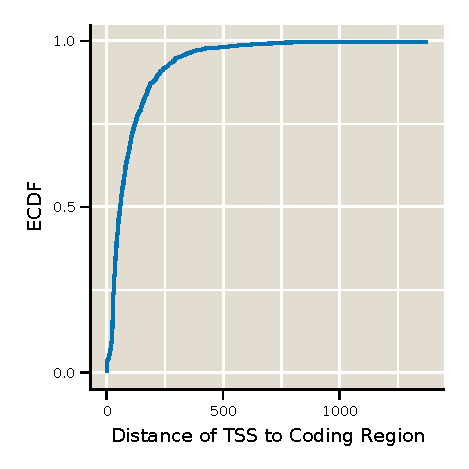
\includegraphics{../figures/tss_CR_distance.pdf}
    \caption{ECDF of distances of transcription start sites to the coding region for every operon in \textit{E. coli} that has a transcription start site annotated in EcoCyc. }
    \label{fig:tss_distance}
\end{figure}


\begin{figure}[H]
    \centering
    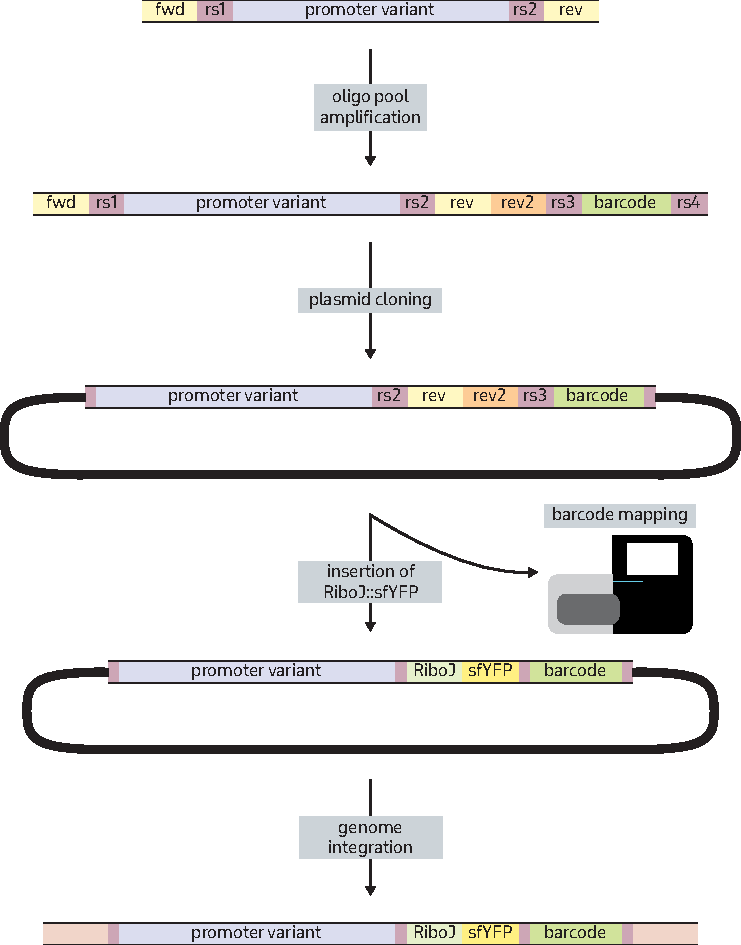
\includegraphics{../figures/cloning_scheme.pdf}
    \caption{Placeholder figure for cloning scheme.}
    \label{fig:cloning}
\end{figure}

\begin{figure}[H]
    \centering
    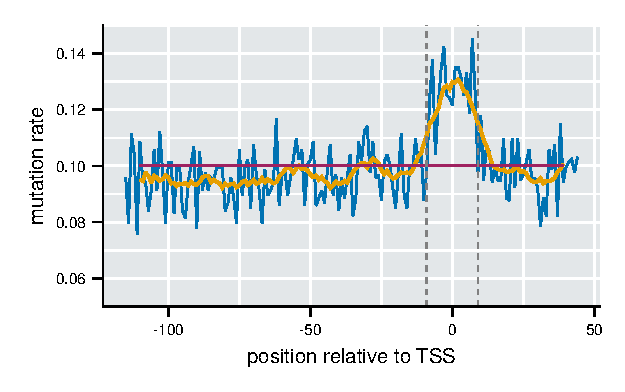
\includegraphics[width=0.6\textwidth]{../figures/dicCp_mutation_rate_oligos.pdf}
    \caption{Mutation rate profile for the promoter of \textit{dicC}. Mutation rate per position (blue) with rolling average over 11 positions (orange) compared to expected average mutation rate of 0.1 (purple). Predicted repressor binding site indicated by grey vertical lines.}
    \label{fig:dicCp}
\end{figure}
		% Print supplemental references changing the title
		\clearpage
		\printbibliography[title={Supplemental References},
		segment=\therefsegment, filter=notother]
	\end{refsegment}

}{} % Close boolean to compile SI
\end{document}
